
% I seguenti commenti speciali impostano:
% 1. 
% 2. PDFLaTeX come motore di composizione;
% 3. tesi.tex come documento principale;
% 4. il controllo ortografico italiano per l'editor.

% !TEX encoding = UTF-8
% !TEX TS-program = pdflatex
% !TEX root = tesi.tex
% !TEX spellcheck = it-IT

\documentclass[10pt,                    % corpo del font principale
               a4paper,                 % carta A4
               twoside,                 % impagina per fronte-retro
               openright,               % inizio capitoli a destra
               english,                 
               italian,                 
               ]{book}    

%**************************************************************
% Importazione package
%************************************************************** 

%\usepackage{amsmath,amssymb,amsthm}    % matematica

\usepackage[T1]{fontenc}                % codifica dei font:
                                        % NOTA BENE! richiede una distribuzione *completa* di LaTeX

\usepackage[utf8]{inputenc}             % codifica di input; anche [latin1] va bene
                                        % NOTA BENE! va accordata con le preferenze dell'editor

\usepackage[english, italian]{babel}    % per scrivere in italiano e in inglese;
                                        % l'ultima lingua (l'italiano) risulta predefinita

\usepackage{bookmark}                   % segnalibri

\usepackage{caption}                    % didascalie

\usepackage{chngpage,calc}              % centra il frontespizio

\usepackage{csquotes}                   % gestisce automaticamente i caratteri (")

\usepackage{emptypage}                  % pagine vuote senza testatina e piede di pagina

\usepackage{epigraph}			% per epigrafi

\usepackage{eurosym}                    % simbolo dell'euro

%\usepackage{indentfirst}               % rientra il primo paragrafo di ogni sezione

\usepackage{graphicx}                   % immagini

\usepackage{hyperref}                   % collegamenti ipertestuali

\usepackage[binding=5mm]{layaureo}      % margini ottimizzati per l'A4; rilegatura di 5 mm

\usepackage{listings}                   % codici

\usepackage{microtype}                  % microtipografia

\usepackage{mparhack,fixltx2e,relsize}  % finezze tipografiche

\usepackage{nameref}                    % visualizza nome dei riferimenti                                      

\usepackage[font=small]{quoting}        % citazioni

\usepackage{subfig}                     % sottofigure, sottotabelle

\usepackage[italian]{varioref}          % riferimenti completi della pagina

\usepackage[dvipsnames]{xcolor}         % colori

\usepackage{booktabs}                   % tabelle                                       
\usepackage{tabularx}                   % tabelle di larghezza prefissata                                    
\usepackage{longtable}                  % tabelle su più pagine                                        
\usepackage{ltxtable}                   % tabelle su più pagine e adattabili in larghezza

\usepackage[toc, acronym]{glossaries}   % glossario
                                        % per includerlo nel documento bisogna:
                                        % 1. compilare una prima volta tesi.tex;
                                        % 2. eseguire: makeindex -s tesi.ist -t tesi.glg -o tesi.gls tesi.glo
                                        % 3. eseguire: makeindex -s tesi.ist -t tesi.alg -o tesi.acr tesi.acn
                                        % 4. compilare due volte tesi.tex.

\usepackage[backend=biber,style=verbose-ibid,hyperref,backref]{biblatex}
                                        % eccellente pacchetto per la bibliografia; 
                                        % produce uno stile di citazione autore-anno; 
                                        % lo stile "numeric-comp" produce riferimenti numerici
                                        % per includerlo nel documento bisogna:
                                        % 1. compilare una prima volta tesi.tex;
                                        % 2. eseguire: biber tesi
                                        % 3. compilare ancora tesi.tex.

%**************************************************************
% file contenente le impostazioni della tesi
%**************************************************************

%**************************************************************
% Frontespizio
%**************************************************************
\newcommand{\source}[1]{\caption*{\textbf{Fonte:} {#1}} }
\newcommand{\AD}{AzzurroDigitale}
\newcommand{\DS}{DigitalSnapshots}

% Autore
\newcommand{\myName}{Luca Stocco}                                    
\newcommand{\myTitle}{Soluzioni digitali nell’ambito Industria 4.0:
AWMS di AzzurroDigitale}

% Tipo di tesi                   
\newcommand{\myDegree}{Tesi di laurea triennale}

% Università             
\newcommand{\myUni}{Università degli Studi di Padova}

% Facoltà       
\newcommand{\myFaculty}{Corso di Laurea in Informatica}

% Dipartimento
\newcommand{\myDepartment}{Dipartimento di Matematica "Tullio Levi-Civita"}

% Titolo del relatore
\newcommand{\profTitle}{Prof.}

% Relatore
\newcommand{\myProf}{Tullio Vardanega}

% Luogo
\newcommand{\myLocation}{Padova}

% Anno accademico
\newcommand{\myAA}{2018-2019}

% Data discussione
\newcommand{\myTime}{18 Dicembre 2019}


%**************************************************************
% Impostazioni di impaginazione
% see: http://wwwcdf.pd.infn.it/AppuntiLinux/a2547.htm
%**************************************************************

\setlength{\parindent}{14pt}   % larghezza rientro della prima riga
\setlength{\parskip}{0pt}   % distanza tra i paragrafi


%**************************************************************
% Impostazioni di biblatex
%**************************************************************
\bibliography{bibliografia} % database di biblatex 

\defbibheading{bibliography} {
    \cleardoublepage
    \phantomsection 
    \addcontentsline{toc}{chapter}{\bibname}
    \chapter*{\bibname\markboth{\bibname}{\bibname}}
}

\setlength\bibitemsep{1.5\itemsep} % spazio tra entry

\DeclareBibliographyCategory{opere}
\DeclareBibliographyCategory{web}

\addtocategory{opere}{womak:lean-thinking}
\addtocategory{web}{site:agile-manifesto}

\defbibheading{opere}{\section*{Riferimenti bibliografici}}
\defbibheading{web}{\section*{Siti Web consultati}}


%**************************************************************
% Impostazioni di caption
%**************************************************************
\captionsetup{
    tableposition=top,
    figureposition=bottom,
    font=small,
    format=hang,
    labelfont=bf
}

%**************************************************************
% Impostazioni di glossaries
%**************************************************************
\loadglsentries{glossario} % database di termini
\makeglossaries


%**************************************************************
% Impostazioni di graphicx
%**************************************************************
\graphicspath{{immagini/}} % cartella dove sono riposte le immagini


%**************************************************************
% Impostazioni di hyperref
%**************************************************************
\hypersetup{
    %hyperfootnotes=false,
    %pdfpagelabels,
    %draft,	% = elimina tutti i link (utile per stampe in bianco e nero)
    %colorlinks=true,
    %linktocpage=true,
    %pdfstartpage=1,
    %pdfstartview=FitV,
    % decommenta la riga seguente per avere link in nero (per esempio per la stampa in bianco e nero)
    colorlinks=false, linktocpage=false, pdfborder={0 0 0}, pdfstartpage=1, pdfstartview=FitV,
    breaklinks=true,
    pdfpagemode=UseNone,
    pageanchor=true,
    pdfpagemode=UseOutlines,
    plainpages=false,
    bookmarksnumbered,
    bookmarksopen=true,
    bookmarksopenlevel=1,
    hypertexnames=true,
    pdfhighlight=/O,
    %nesting=true,
    %frenchlinks,
    urlcolor=webbrown,
    linkcolor=RoyalBlue,
    citecolor=webgreen,
    %pagecolor=RoyalBlue,
    %urlcolor=Black, linkcolor=Black, citecolor=Black, %pagecolor=Black,
    pdftitle={\myTitle},
    pdfauthor={\textcopyright\ \myName, \myUni, \myFaculty},
    pdfsubject={},
    pdfkeywords={},
    pdfcreator={pdfLaTeX},
    pdfproducer={LaTeX}
}

%**************************************************************
% Impostazioni di itemize
%**************************************************************
%\renewcommand{\labelitemi}{$\ast$}

%\renewcommand{\labelitemi}{$\bullet$}
%\renewcommand{\labelitemii}{$\cdot$}
%\renewcommand{\labelitemiii}{$\diamond$}
%\renewcommand{\labelitemiv}{$\ast$}


%**************************************************************
% Impostazioni di listings
%**************************************************************
\lstset{
    language=[LaTeX]Tex,%C++,
    keywordstyle=\color{RoyalBlue}, %\bfseries,
    basicstyle=\small\ttfamily,
    %identifierstyle=\color{NavyBlue},
    commentstyle=\color{Green}\ttfamily,
    stringstyle=\rmfamily,
    numbers=none, %left,%
    numberstyle=\scriptsize, %\tiny
    stepnumber=5,
    numbersep=8pt,
    showstringspaces=false,
    breaklines=true,
    frameround=ftff,
    frame=single
} 


%**************************************************************
% Impostazioni di xcolor
%**************************************************************
\definecolor{webgreen}{rgb}{0,.5,0}
\definecolor{webbrown}{rgb}{.6,0,0}


%**************************************************************
% Altro
%**************************************************************

\newcommand{\omissis}{[\dots\negthinspace]} % produce [...]

% eccezioni all'algoritmo di sillabazione
\hyphenation
{
    ma-cro-istru-zio-ne
    gi-ral-din
}

\newcommand{\sectionname}{sezione}
\addto\captionsitalian{\renewcommand{\figurename}{Figura}
                       \renewcommand{\tablename}{Tabella}}

\newcommand{\markg}[1]{#1\ped{g}}

\newcommand{\intro}[1]{\emph{\textsf{#1}}}

%**************************************************************
% Environment per ``rischi''
%**************************************************************
\newcounter{riskcounter}                % define a counter
\setcounter{riskcounter}{0}             % set the counter to some initial value

%%%% Parameters
% #1: Title
\newenvironment{risk}[1]{
    \refstepcounter{riskcounter}        % increment counter
    \par \noindent                      % start new paragraph
    \textbf{\arabic{riskcounter}. #1}   % display the title before the 
                                        % content of the environment is displayed 
}{
    \par\medskip
}

\newcommand{\riskname}{Rischio}

\newcommand{\riskdescription}[1]{\textbf{\\Descrizione:} #1.}

\newcommand{\risksolution}[1]{\textbf{\\Soluzione:} #1.}

%**************************************************************
% Environment per ``use case''
%**************************************************************
\newcounter{usecasecounter}             % define a counter
\setcounter{usecasecounter}{0}          % set the counter to some initial value

%%%% Parameters
% #1: ID
% #2: Nome
\newenvironment{usecase}[2]{
    \renewcommand{\theusecasecounter}{\usecasename #1}  % this is where the display of 
                                                        % the counter is overwritten/modified
    \refstepcounter{usecasecounter}             % increment counter
    \vspace{10pt}
    \par \noindent                              % start new paragraph
    {\large \textbf{\usecasename #1: #2}}       % display the title before the 
                                                % content of the environment is displayed 
    \medskip
}{
    \medskip
}

\newcommand{\usecasename}{UC}

\newcommand{\usecaseactors}[1]{\textbf{\\Attori Principali:} #1. \vspace{4pt}}
\newcommand{\usecasepre}[1]{\textbf{\\Precondizioni:} #1. \vspace{4pt}}
\newcommand{\usecasedesc}[1]{\textbf{\\Descrizione:} #1. \vspace{4pt}}
\newcommand{\usecasepost}[1]{\textbf{\\Postcondizioni:} #1. \vspace{4pt}}
\newcommand{\usecasealt}[1]{\textbf{\\Scenario Alternativo:} #1. \vspace{4pt}}

%**************************************************************
% Environment per ``namespace description''
%**************************************************************

\newenvironment{namespacedesc}{
    \vspace{10pt}
    \par \noindent                              % start new paragraph
    \begin{description} 
}{
    \end{description}
    \medskip
}

\newcommand{\classdesc}[2]{\item[\textbf{#1:}] #2}                     % file con le impostazioni personali

\begin{document}
%**************************************************************
% Materiale iniziale
%**************************************************************
\frontmatter
% !TEX encoding = UTF-8
% !TEX TS-program = pdflatex
% !TEX root = ../tesi.tex

%**************************************************************
% Frontespizio 
%**************************************************************
\begin{titlepage}

\begin{center}

\begin{LARGE}
\textbf{\myUni}\\
\end{LARGE}

\vspace{10pt}

\begin{Large}
\textsc{\myDepartment}\\
\end{Large}

\vspace{10pt}

\begin{large}
\textsc{\myFaculty}\\
\end{large}

\vspace{30pt}
\begin{figure}[htbp]
\begin{center}

\includegraphics[height=6cm]{logo-unipd}
\end{center}
\end{figure}
\vspace{30pt} 

\begin{LARGE}
\begin{center}
\textbf{\myTitle}\\
\end{center}
\end{LARGE}

\vspace{10pt} 

\begin{large}
\textsl{\myDegree}\\
\end{large}

\vspace{40pt} 

\begin{large}
\begin{flushleft}
\textit{Relatore}\\ 
\vspace{5pt} 
\profTitle \myProf
\end{flushleft}

\vspace{0pt} 

\begin{flushright}
\textit{Laureando}\\ 
\vspace{5pt} 
\myName
\end{flushright}
\end{large}

\vspace{40pt}

\line(1, 0){338} \\
\begin{normalsize}
\textsc{Anno Accademico \myAA}
\end{normalsize}

\end{center}
\end{titlepage} 
% !TEX encoding = UTF-8
% !TEX TS-program = pdflatex
% !TEX root = ../tesi.tex

%**************************************************************
% Colophon
%**************************************************************
\cleardoublepage
\phantomsection
\thispagestyle{empty}

\hfill

\vfill

\noindent\myName: \textit{\myTitle,}
\myDegree,
\textcopyright\ \myTime.
% !TEX encoding = UTF-8
% !TEX TS-program = pdflatex
% !TEX root = ../tesi.tex

%**************************************************************
% Dedica
%**************************************************************
\cleardoublepage
\phantomsection
\thispagestyle{empty}
\pdfbookmark{Dedica}{Dedica}

\vspace*{3cm}

\begin{center}
Lorem ipsum dolor sit amet, consectetuer adipiscing elit. \\ \medskip
--- Oscar Wilde    
\end{center}

\medskip

\begin{center}
Dedicato a ...
\end{center}

% !TEX encoding = UTF-8
% !TEX TS-program = pdflatex
% !TEX root = ../tesi.tex

%**************************************************************
% Sommario
%**************************************************************
\cleardoublepage
\phantomsection
\pdfbookmark{Sommario}{Sommario}
\begingroup
\let\clearpage\relax
\let\cleardoublepage\relax
\let\cleardoublepage\relax

\chapter*{Sommario}
\section*{Organizzazione del testo}

\begin{description}
    \item[{\hyperref[cap:introduzione]{Il primo capitolo}}] descrive ...
    
    \item[{\hyperref[cap:obiettivi-stage]{Il secondo capitolo}}] descrive ...
    
    \item[{\hyperref[cap:descrizione-stage]{Il terzo capitolo}}] approfondisce ...
    
    \item[{\hyperref[cap:analisi-requisiti]{Il quarto capitolo}}] approfondisce ...
\end{description}
 
Riguardo la stesura del testo, relativamente al documento sono state adottate le seguenti convenzioni tipografiche:
\begin{itemize}
	\item gli acronimi, le abbreviazioni e i termini ambigui o di uso non comune menzionati vengono definiti nel glossario, situato alla fine del presente documento;
	\item per la prima occorrenza dei termini riportati nel glossario viene utilizzata la seguente nomenclatura: \emph{parola}\glsfirstoccur;
	\item i termini in lingua straniera o facenti parti del gergo tecnico sono evidenziati con il carattere \emph{corsivo}.
\end{itemize}

%\vfill
%
%\selectlanguage{english}
%\pdfbookmark{Abstract}{Abstract}
%\chapter*{Abstract}
%
%\selectlanguage{italian}

\endgroup			

\vfill


% !TEX encoding = UTF-8
% !TEX TS-program = pdflatex
% !TEX root = ../tesi.tex

%**************************************************************
% Ringraziamenti
%**************************************************************
\cleardoublepage
\phantomsection
\pdfbookmark{Ringraziamenti}{ringraziamenti}

\begin{flushright}{
	\slshape    
	``Then you better start swimmin’ or you’ll sink like a stone\\For the times they are a-changin’
''} \\ 
	\medskip
    --- Bob Dylan
\end{flushright}


\bigskip

\begingroup
\let\clearpage\relax
\let\cleardoublepage\relax
\let\cleardoublepage\relax

\chapter*{Ringraziamenti}

\noindent \textit{Innanzitutto, vorrei esprimere la mia gratitudine al \profTitle \myProf, relatore della mia tesi, per l'aiuto e il sostegno fornitomi durante la stesura del lavoro.}\\

\noindent \textit{Desidero ringraziare con affetto i miei genitori per il sostegno, il grande aiuto e per essermi stati vicini in ogni momento durante gli anni di studio.}\\

\noindent \textit{Ho desiderio di ringraziare poi i miei amici per tutti i bellissimi anni passati insieme e le mille avventure vissute.}\\
\bigskip

\noindent\textit{\myLocation, \myTime}
\hfill \myName

\endgroup


% !TEX encoding = UTF-8
% !TEX TS-program = pdflatex
% !TEX root = ../tesi.tex

%**************************************************************
% Indici
%**************************************************************
\cleardoublepage
\pdfbookmark{\contentsname}{tableofcontents}
\setcounter{tocdepth}{2}
\tableofcontents
%\markboth{\contentsname}{\contentsname} 
\clearpage

\begingroup 
    \let\clearpage\relax
    \let\cleardoublepage\relax
    \let\cleardoublepage\relax
    %*******************************************************
    % Elenco delle figure
    %*******************************************************    
    \phantomsection
    \pdfbookmark{\listfigurename}{lof}
    \listoffigures

    \vspace*{8ex}

    %*******************************************************
    % Elenco delle tabelle
    %*******************************************************
    \phantomsection
    \pdfbookmark{\listtablename}{lot}
    \listoftables
        
    \vspace*{8ex}
\endgroup

\cleardoublepage

\cleardoublepage

%**************************************************************
% Materiale principale
%**************************************************************
\mainmatter
% !TEX encoding = UTF-8
% !TEX TS-program = pdflatex
% !TEX root = ../tesi.tex
\newpage
%**************************************************************
\chapter{Contesto Aziendale}
\label{cap:introduzione}

\section{L'azienda}
\AD{} è una start-up nata nel 2014, dall'idea di tre giovani padovani, Carlo Pasqualetto, Jacopo Pertile e Antonio Fornari, con l'intento di assistere le aziende nel miglioramento e nella digitalizzazione dei propri processi interni.\\
Inizialmente, \AD{} si rivolgeva ad un pubblico formato da piccole e medie imprese, fornendo loro consulenze di strategie aziendali, formazione del personale sugli strumenti digitali da utilizzare e piccoli software su misura.\\
Il salto di qualità avviene del 2016, quando \AD{} partecipa ad una competizione organizzata dal colosso svedese degli elettrodomestici Electrolux, per sviluppare un progetto di pianificazione intelligente della forza lavoro.

\begin{figure}[h]

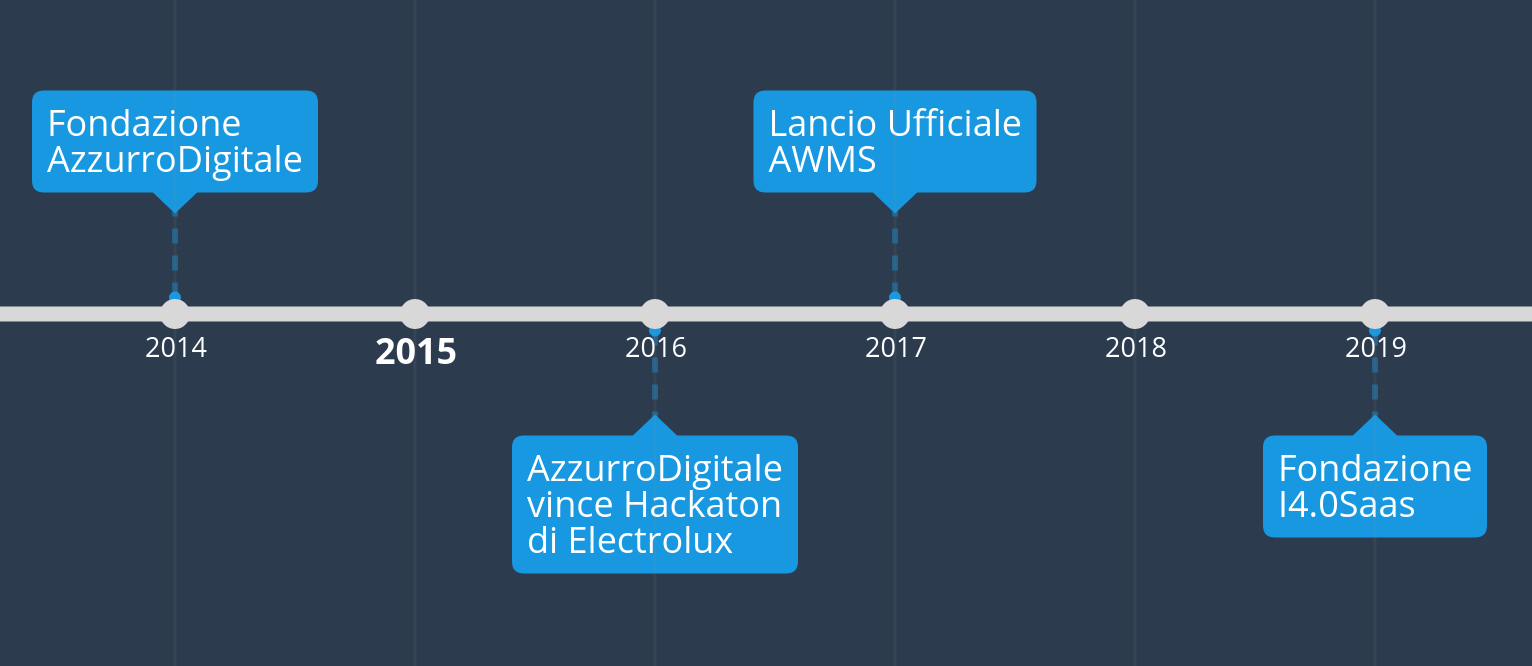
\includegraphics[width=0.8\textwidth]{AD_timeline.png}
\centering
\caption{Punti focali della storia di \AD{}.}
\end{figure}
La vittoria di questa competizione, ha portato alla nascita del progetto AWMS, prodotto di punta di \AD{}.\\
Vista la grossa richiesta di AWMS da parte di importanti aziende nazionali ed internazionali, nel 2019 i tre soci decidono di dare vita ad \textbf{I4.0Saas}, uno \textit{spin-off} di \AD{}, che a partire dal 2020 si occuperà esclusivamente della gestione e dello sviluppo del progetto AWMS.\\

\subsection{Obiettivi e valori}
%descrizione degli obiettivi (ovvero DOVE l'azienda sta puntando ad arrivare) e i valori cardine dell'azienda (Azzurrite)\\

%%%%%%%%%%%%%%%%%%%%%%%%%%%%%%%%%%%%%%%%%%%%%%%%%%%%%%%%%%%%%%%%%%%%%%%%%%%%%%%%%%%%%%%%%%%
Il valore cardine sul quale si fonda \AD{} è la \textbf{voglia di innovazione}, requisito fondamentale per un'azienda che opera nell'ambito della \textit{digital transformation}.

\AD{} si è posta, fin dalla nascita, l'obiettivo di entrare con le proprie soluzioni nelle maggiori aziende manifatturiere mondiali. 

%%%%%%%%%%%%%%%%%%%%%%%%%%%%%%%%%%%%%%%%%%%%%%%%%%%%%%%%%%%%%%%%%%%%%%%%%%%%%%%%%%%%%%%%%%%



\subsection{Modello di business}
%descrizione del modello di business (AzzurroDigitale: strategies and ventures)\\
Il modello di business principale di \AD{} si orienta fondamentalmente sulla \textit{digital transformation} delle aziende.
In questo frangente, nello specifico, \AD{} opera in due settori:
\begin{itemize}
\item \textbf{Gestione della forza lavoro:} ovvero la pianificazione ottimale delle risorse umane all'interno di un reparto produttivo;
\item \textbf{Digitalizzazione dei processi aziendali:} ovvero la trasposizione in maniera automatica e digitale di tutte le attività di un processo che in precedenza venivano effettuate manualmente o in maniera non automatizzata, così da migliorare l'efficienza del processo stesso. 
\end{itemize}
\begin{figure}[h]
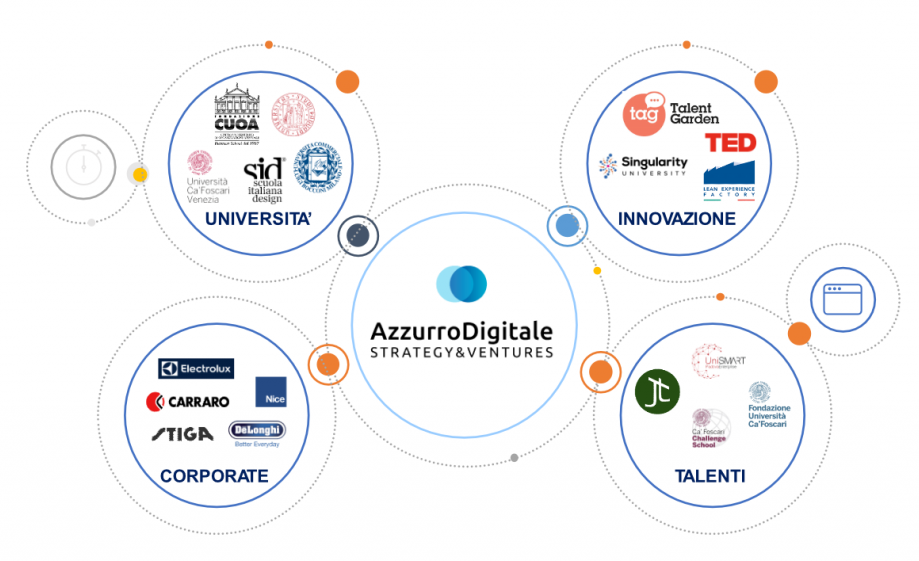
\includegraphics[width=\textwidth]{AD-network.png}
\centering
\caption{Innovation Network di AzzurroDigitale.} 
\source{\href{https://www.azzurrodigitale.com/}{Azzurrodigitale.com}}
\label{fig:innovation-network}
\end{figure}
Lavorando a stretto contatto con l'ambiente universitario, \AD{} organizza anche laboratori didattici interattivi, nei quali gli studenti si troveranno ad affrontare alcune delle sfide del mondo lavorativo, proposte da aziende partner.

\subsection{Prodotti e \textit{spin-off}}
%- panoramica sulle tipologie di prodotti realizzate (trasformazione digitale delle aziende)\\
%- spin-off: I4.0Saas\\
I prodotti realizzati da \AD{} riguardano, come accennato, il settore manifatturiero e la gestione della forza lavoro.
Sin dalla sua nascita infatti, \AD{} ha offerto ai propri clienti, software su misura per il monitoraggio e per il miglioramento dei processi legati al reparto di produzione.\\
Tra questi, è necessario citare \textit{Digital Cockpit}: una webapp sviluppata in collaborazione con Safilo, azienda tra i leader mondiali nella produzione di occhiali.\\
Si tratta di un'applicazione che monitora i macchinari del reparto produzione e ne registra tutti i parametri di lavoro, fornendo così un cruscotto informativo completo sull'efficienza giornaliera del macchinario, oltre alle tempistiche di lavoro, ai dettagli del prodotto in fase di lavorazione e ai tempi morti del macchinario stesso.\\
Aumentando il numero di clienti, \AD{} ha cominciato a sviluppare anche software non legati al singolo cliente, rimanendo sempre nell'ambito della \textit{digital transformation}:
\begin{itemize}
\item \textbf{AWMS:} \textit{Advanced Workforce Management System} è una soluzione software che, tramite algoritmi di \textit{machine learning}, si occupa di pianificare in maniera ottimale la forza lavoro all'interno di uno stabilimento produttivo, tenendo conto di assenze inaspettate, livello di esperienza dell'operatore in una determinata mansione e certificazioni in possesso di quest'ultimo. \\
Si tratta del prodotto di punta di \AD{} ed attualmente figurano tra i suoi utilizzatori, aziende rinomate come Electrolux, Safilo Group, Zoppas Industries, Stiga e Ferrari;
\item \textbf{DigitalSnapshots:} Software sviluppato in collaborazione con Electrolux, ha lo scopo di monitorare lo stato di avanzamento dei progetti all'interno dei vari stabilimenti, fornendo così una panoramica sulle risorse impegnate e/o mancanti nei singoli progetti, la percentuale di avanzamento del progetto stesso, ed il peso in termini di importanza che quel progetto ha all'interno dello stabilimento.
\end{itemize}

\subsubsection*{\textit{Spin-off}}
Come accennato ad inizio capitolo, nel corso del 2019 è nata \textbf{I4.0Saas}, ovvero un distaccamento di \AD{} che a partire dal 2020 andrà ad occuparsi della vendita, della gestione e dello sviluppo del software AWMS.

\section{Organizzazione interna}
%Organizzazione aziendale: team sviluppo e team consulenze. Descrizione dettagliata di entrambi
Come descritto in precedenza, \AD{} crede fortemente nel capitale umano e nello spirito di squadra. Per questo motivo, all'interno di essa non esiste una netta gerarchia del personale: ogni dipendente è considerato alla pari, ed ogni idea o proposta viene discussa e valutata senza pregiudizio. \\
Tuttavia, il personale può essere suddiviso in base alle competenze e alla propria mansione all'interno dell'azienda. Possiamo quindi trovare i seguenti reparti:
\begin{itemize}
\item \textbf{\textit{Development}}\\
Questo reparto ha il compito di sviluppare il prodotto, definendo ed implementando tutte le caratteristiche accordate con il cliente, sia a livello logico (\textit{back-end}) che a livello visuale (\textit{front-end}). Fa parte di questo reparto anche la figura del designer, che ha il compito di definire l'interfaccia utente alla quale poi gli sviluppatori dovranno far riferimento;  
\item \textbf{\textit{Consulting}}\\
Questo è un reparto chiave per il modello di business di \AD{}. E\` formato da consulenti che hanno lo scopo di analizzare i processi aziendali dei clienti, individuare le inefficienze e proporre delle soluzioni o delle strategie affinché venga massimizzata l'efficienza dello stabilimento. Inoltre, svolgono il ruolo di analista funzionale, che si pone tra il cliente e il team di sviluppo, così da facilitare l'implementazione delle funzionalità richieste;
\item \textbf{\textit{Human Resources} e \textit{Formation}}\\
I membri del reparto delle risorse umane hanno un duplice compito in azienda: in primis, si occupano di contattare, valutare ed eventualmente inserire nuovi innesti nei vari reparti. Inoltre, si dedicano alla preparazione di eventi sulla formazione del personale;
\item \textbf{Amministrazione, Finanza e Controllo}\\
Questo reparto si occupa della parte economica dell'azienda, gestendo il personale, le spese e i ricavi, verificando inoltre il corretto andamento di tutti i reparti.
\end{itemize}

\section{Processi Aziendali}
%metodologia scrum applicata sia nel team sviluppo, sia nel team consulenze
Un'adeguata organizzazione interna è fondamentale per raggiungere gli obiettivi e per offrire ai clienti dei servizi adeguati. Pertanto è richiesta la coordinazione tra tutti i reparti, in modo da raggiungere lo scopo aziendale comune.

\subsubsection*{Comunicazione}
Le comunicazioni interne all'azienda e con i clienti, avvengono prevalentemente tramite e-mail aziendale, così da rendere i contenuti più tracciabili.\\
Per le comunicazioni più informali ed immediate, invece, si utilizzano software di messaggistica istantanea, quali \textit{Slack}, utilizzato soprattutto nel reparto di sviluppo in quanto permette la creazione di canali di comunicazione specifici per ogni progetto, e \textit{Telegram}, per le comunicazioni generali.

\subsubsection*{Gestione di progetto}
Per la gestione del progetto, l'azienda si avvale di molteplici strumenti, a seconda delle diverse fasi ed esigenze:
\begin{itemize}

\item \textbf{Microsoft Office:} Per tutta la documentazione, dalle offerte al tracciamento dei requisiti, passando per la manualistica, viene utilizzata la suite Office di Microsoft;

\item \textbf{Asana:} Questa applicazione viene utilizzata dal \textit{Project Manager} per l'amministrazione della pianificazione. Essa permette infatti di coordinare le risorse, gestire i task e creare i diagrammi di Gantt, a supporto di uno specifico progetto;

\item \textbf{Time Report:} Si tratta di un software sviluppato internamente, viene utilizzato per organizzare e tenere traccia delle ore svolte dai singoli dipendenti per ogni commessa a loro assegnata. Grazie alla sua integrazione con un \textit{bot} di \textit{Telegram}, viene utilizzato anche per la segnalazione rapida delle assenze o dei giorni di ferie;

\item \textbf{Google Calendar:} Questo servizio viene utilizzato per indicare gli impegni di ogni dipendente, in modo da avere una panoramica sulla disponibilità di risorse umane. In aggiunta, viene utilizzato anche per la prenotazione della sala riunioni.
\end{itemize}

\subsubsection*{Sviluppo}
La metodologia di sviluppo adottata nell'azienda riguarda il \textbf{modello Agile} i cui principi sono riassunti nel Manifesto Agile\footnote{\textit{Manifesto Agile.} URL: \href{http://agilemanifesto.org/iso/it/}{http://agilemanifesto.org/iso/it/}}. 
Nello specifico, viene seguito il \textit{framework} Scrum, sintetizzato in figura \ref{fig:scrum}.
Il progetto viene dunque suddiviso in più fasi, dette Sprint. L'obiettivo di ogni Sprint, chiamato Sprint Goal, è quello di portare un prodotto non finito, ma potenzialmente completo e funzionante, secondo gli avanzamento pianificati per il singolo ciclo. Il susseguirsi di questi cicli di durata fissa, nel mio caso di due settimane, porta incrementi al prodotto fino a che questo non soddisfi tutti i requisiti delineati.
Il \textit{framework} Scrum è caratterizzato da una serie di attività prestabilite:
\begin{itemize}
\item \textbf{Product Backlog:} ovvero una lista di tutte le attività, funzionalità e requisiti del prodotto;
\item \textbf{Sprint Planning:} si tratta di una riunione svolta all'inizio di ogni Sprint, ed ha lo scopo di definire gli obiettivi da raggiungere (Sprint Goal) e di pianificare le modalità di come portarli a termine (Sprint Backlog);
\item \textbf{Daily Scrum:} riunione giornaliera in cui il team di sviluppo si aggiorna su cosa è stato fatto il giorno precedente, cosa verrà fatto nelle successive ore lavorative ed eventuali difficoltà affrontate. Lo scopo principale del Daily Scrum è semplificare la collaborazione e l'allineamento del lavoro, e di risolvere eventuali problemi di avanzamento in maniera tempestiva;
\item \textbf{Sprint Review:} Alla fine dello Sprint si tiene l'incontro di Sprint Review per ispezionare l'incremento e adattare, se necessario, il Product Backlog. Durante la riunione di Sprint Review il Team di Sviluppo e gli \textit{stakeholder} collaborano su ciò che è stato fatto durante lo Sprint. In conformità a questo e dei cambiamenti al Product Backlog fatti durante lo Sprint, i partecipanti collaborano sulle prossime cose che potrebbero esser fatte. Si tratta di un incontro informale e la presentazione dell'Incremento ha lo scopo di suscitare commenti e promuovere la collaborazione;
\item \textbf{Sprint Retrospective:} La Sprint Retrospective è l'occasione per il Team Scrum per ispezionare se stesso e creare un piano di miglioramento da attuare durante il prossimo Sprint.
\end{itemize}
\begin{figure}[h]

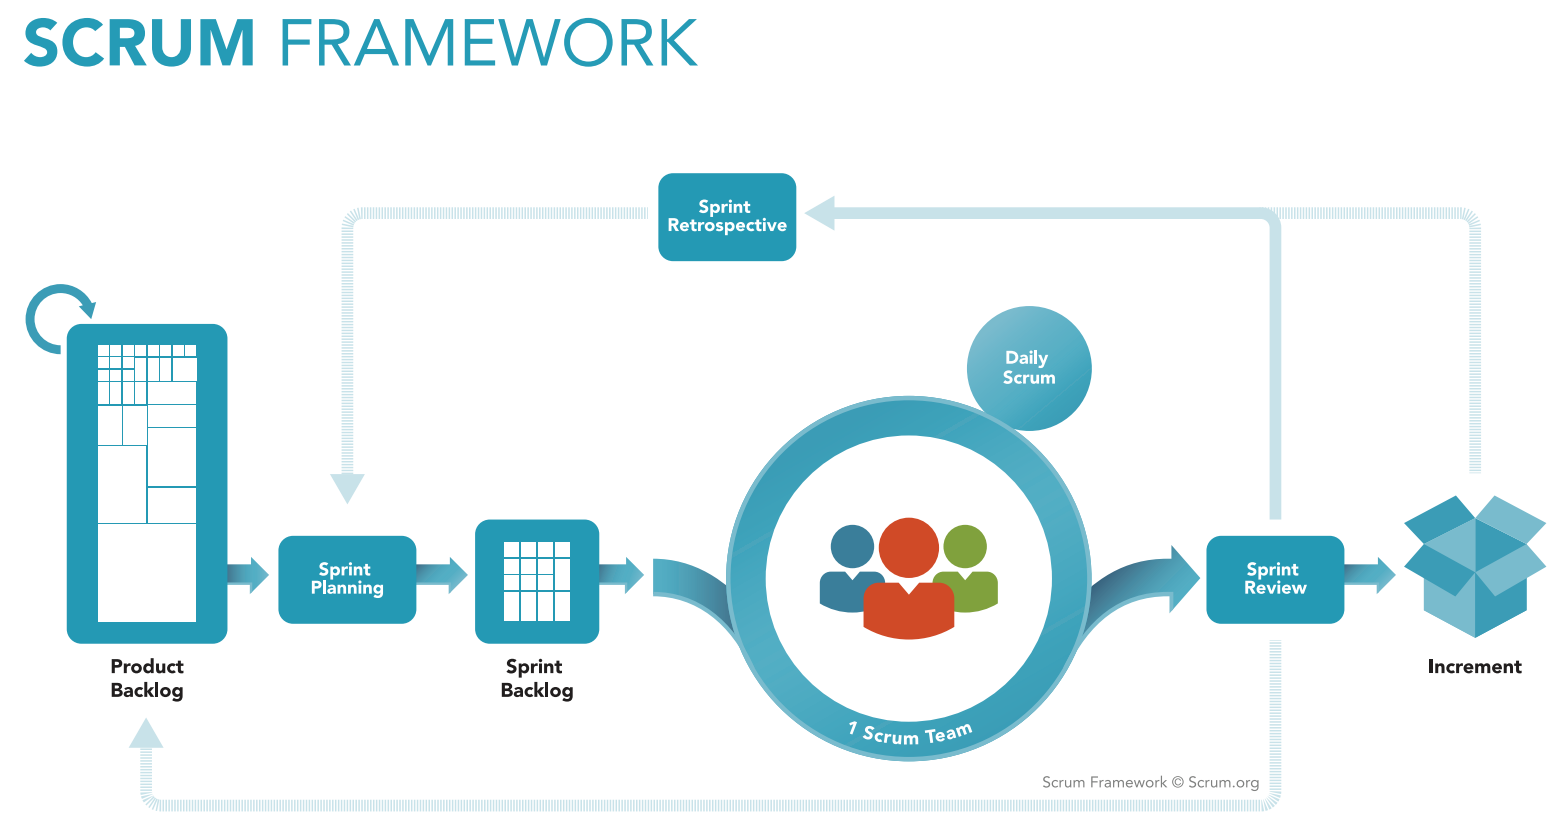
\includegraphics[width=\textwidth]{agile-scrum.png}
\centering
\caption{Rappresentazione del \textit{framework} Scrum.}
\source{\href{https://www.scrum.org/}{Scrum.org}}
\label{fig:scrum}
\end{figure}
\AD{} ha deciso di adottare la metodologia agile per lo sviluppo software in quanto permette all'azienda di essere molto elastica rispetto ad eventuali cambiamenti dei requisiti iniziali, oltre che a permettere il \textit{deploy} di un prodotto non finito, ma potenzialmente completo e funzionante al termine di ogni Sprint, riuscendo così ad avere un \textit{feedback} sul prodotto nel minor tempo possibile.  

\subsubsection*{\textit{Consulting}}
A differenza del reparto di sviluppo, il reparto di \textit{consulting} ha adottato un approccio lavorativo originale, studiato e realizzato in collaborazione con il dipartimento di Ingegneria Gestionale dell’Università di Padova, chiamato \textbf{\textit{"The digitalization factory loop"}}.\\
\`E possibile riassumere questo approccio in tre semplici frasi, ognuna delle quali corrisponde ad una fase del processo, \textit{“Make it Clear, Make it Tangible, Make it Real”}.

\begin{figure}[h]

\includegraphics[width=\textwidth]{makeitreal.png}
\centering
\caption{Rappresentazione del \textit{digitalization factory loop}.} 
\source{\href{https://www.azzurrodigitale.com/}{Azzurrodigitale.com}}

\label{fig:make-it-real}
\end{figure}
Questo approccio dunque, consiste nello scomporre il processo in 3 fasi distinte e ripeterle fino al raggiungimento dell'obiettivo:
\begin{itemize}
\item \textbf{\textit{Make it clear}:} in questa fase si definiscono degli obiettivi digitali prioritari cercando di comprendere come la tecnologia può essere utilizzata per il successo aziendale e in che modo è bene indirizzare gli investimenti;
\item \textbf{\textit{Make it Tangible}:} dagli obiettivi digitali si passa ai progetti digitali, così da definire in modo tangibile la strategia digitale. In questo step dei team operativi composti da impiegati verranno creati per generare la strategia;
\item \textbf{\textit{Make it Real}:} in questa fase i progetti vengono concretamente realizzati attraverso un’implementazione day-by-day e la coordinazione dei team di lavoro con specifiche metodologie di project management.
\end{itemize}             % Introduzione
% !TEX encoding = UTF-8
% !TEX TS-program = pdflatex
% !TEX root = ../tesi.tex
\newpage
%**************************************************************
\chapter{Obiettivi dello stage}
\label{cap:obiettivi-stage}
%\intro{Brevissima introduzione al capitolo}\\
%%%%%%%%%%%%%%%%%%%%%%%%%%%%%%%%%%%%%%%%%%%%%%%%%%%%%%%%%%%%%%%%%%%%%%%%%%%%%%%%%%%%%%%%%%%
\section{Lo stage nella strategia aziendale}
%Importanza dello stage in AzzurroDigitale
%%%%%%%%%%%%%%%%%%%%%%%%%%%%%%%%%%%%%%%%%%%%%%%%%%%%%%%%%%%%%%%%%%%%%%%%%%%%%%%%%%%%%%%%%%%
\subsection{Vantaggi Aziendali}
%Vantaggi per l'azienda: \\
%- partecipazione a stageIT consente all'azienda di entrare in contatto con i laureandi\\
%- formazione di personale giovane e selezionato\\
%- nuove idee e punti di vista \\
%%%%%%%%%%%%%%%%%%%%%%%%%%%%%%%%%%%%%%%%%%%%%%%%%%%%%%%%%%%%%%%%%%%%%%%%%%%%%%%%%%%%%%%%%%%
\subsection{Presentazione dei progetti}
%descrizione generale dei progetti: \\
%- le idee che stanno dietro a questi\\
%- peculiarità\\
%- differenze con la concorrenza\\
%%%%%%%%%%%%%%%%%%%%%%%%%%%%%%%%%%%%%%%%%%%%%%%%%%%%%%%%%%%%%%%%%%%%%%%%%%%%%%%%%%%%%%%%%%%

\begin{figure}[h]
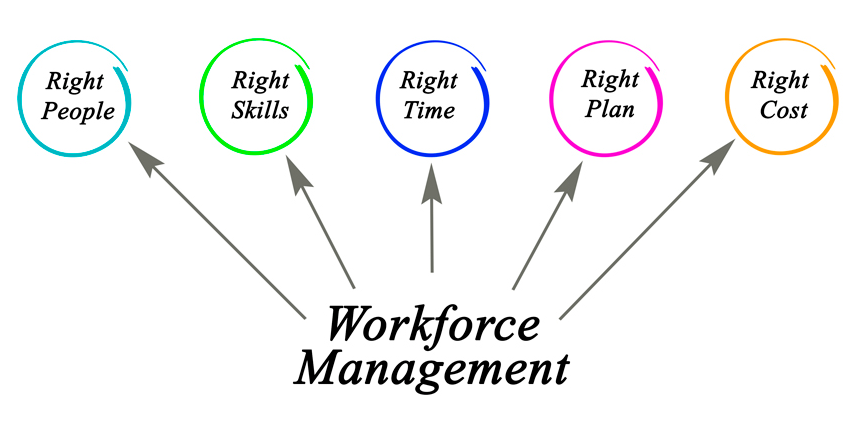
\includegraphics[width=0.9\textwidth]{workforce-management.png}
\centering
\caption{Concetti di \textit{Workforce Management}.} 
\source{\href{https://www.replgroup.com/}{Replgroup.com}}
\label{fig:workforce-management}
\end{figure}


\subsection{Aspettative aziendali}
%definizione e classificazione degli obiettivi da raggiungere

Presentati i progetti, si è passati alla fase di definizione dei traguardi da raggiungere durante lo stage.
Il team di sviluppo ha deciso di suddividere questi obiettivi in due categorie: gli \textbf{obiettivi minimi} si riferiscono a dei compiti il cui completamento risulta essere indispensabile per l'avanzamento del progetto, gli \textbf{obiettivi opzionali} invece, fanno riferimento a delle caratteristiche del prodotto di importanza minore e quindi il loro soddisfacimento non è stato considerato obbligatorio.
Di seguito, il riepilogo degli obiettivi che mi sono stati assegnati, ripartiti tra i vari progetti.

\subsubsection*{DigitalSnapshots}
\paragraph*{Obiettivi Minimi}
\begin{itemize}
\item Ristrutturazione della base di dati MySQL e della parte Model di CakePHP;
\item Realizzazione moduli API e logica;
\item Creazione interfaccia utente del cruscotto delle analisi; 
\item Stesura della documentazione su quanto realizzato.
\end{itemize}

\paragraph*{Obiettivi Opzionali}
\begin{itemize}
\item Realizzazione di un modulo \textit{wizard} per la configurazione rapida del prodotto;
\item Implementazione di una gerarchia di utenti, con livelli di privilegi differenti.
\end{itemize}

\subsubsection*{AWMS}
\paragraph*{Obiettivi Minimi}
\begin{itemize}
\item Implementazione dei dati necessari nel database PostgreSQL e nella parte Model di CakePHP;
\item Realizzazione moduli API e logica;
\item Creazione interfaccia utente per la selezione della tipologia e delle opzioni di stampa; 
\item Stesura della documentazione su quanto realizzato.
\end{itemize}

\paragraph*{Obiettivi Opzionali}
\begin{itemize}
\item Realizzazione di un modulo per la configurazione dei ruoli degli utenti;
\item Implementazione di un algoritmo per la pianificazione intelligente della forza lavoro a disposizione.
\end{itemize}

\section{Vincoli}
\subsection{Vincoli temporali}
%ore di lavoro complessive, scadenze sprint e scadenze di progetto

La durata complessiva dell'attività di stage è stata di 304 ore, distribuite, in accordo con il tutor aziendale, nell'arco di 8 settimane, ognuna delle quali aveva un monte orario di circa 40 ore. \\
L'orario lavorativo stabilito corrisponde all'orario di lavoro aziendale: dal Lunedì al Venerdi, dalle ore 9:00 alle 18:00.\\
Oltre a questo vincolo del monte orario, mi sono trovato a toccare con mano la pianificazione Scrum: all'inizio di ogni Sprint, infatti, ho pianificato le attività da portare a termine entro le successive due settimane, durata di ogni singolo Sprint.//
Il progetto \textbf{DigitalSnapshots} inoltre, aveva una scadenza di consegna al cliente che combaciava con la fine del secondo Sprint, per cui il ritmo lavorativo è stato abbastanza elevato per non eccedere tale data.

\begin{figure}[h]
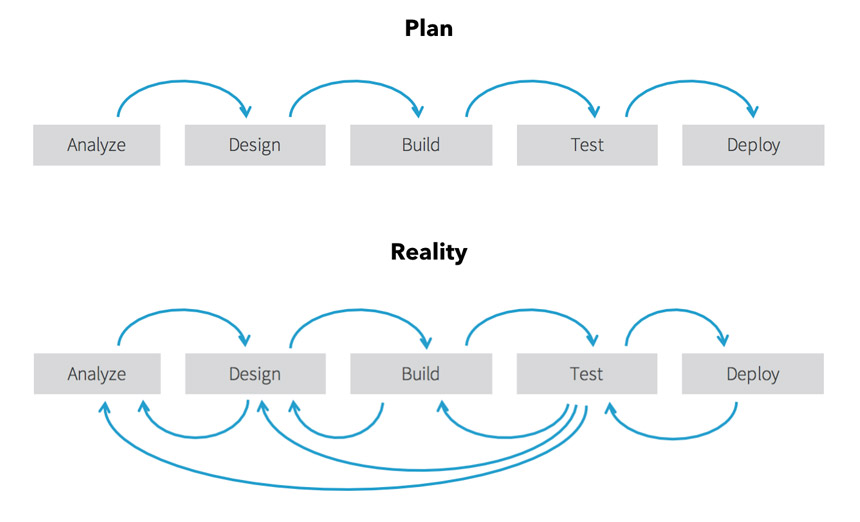
\includegraphics[width=\textwidth , keepaspectratio]{plan-vs-reality.jpg}
\centering
\caption{Rischi di pianificazione nell'attività di codifica.} 
\source{\href{https://www.devbridge.com/}{Devbridge.com}}
\label{fig:plan-vs-reality}
\end{figure}

\subsection{Vincoli metodologici}
%- monday meeting\\
%- interazione diretta con il cliente\\
%- scrum\\
%- Vincoli metodologici personali
Al mio arrivo in azienda, il progetto già presentava un'architettura e una metodologia di lavoro consolidate.
Data la mia poca esperienza con il \textit{framework} Scrum, in accordo unanime tra tutto il team, abbiamo deciso di mantenere la durata degli Sprint pari a due settimane lavorative, ma di inserire a metà di questo lasso di tempo una riunione che aveva la funzione di monitorare l'andamento dello sviluppo e di rilevarne eventuali criticità. I \textit{meeting} di \textit{Sprint Review} erano spesso presenziati anche dal comparto tecnico o dalle persone di riferimento delle aziende \textit{stakeholder}, così da avere un \textit{feedback} su quanto fatto finora pressoché istantaneo.
A questi inoltre, si aggiunge la politica aziendale del \textit{Monday Meeting}, ovvero una assemblea, effettuata ogni due Lunedì, nel corso del quale si aggiornano i colleghi sull'andamento dei progetti in corso.
Nonostante avessi carta bianca sulla modalità di sviluppo del codice, mi sono posto dei vincoli da rispettare, affinchè l'attività risultasse il più efficiente ed efficace possibile.\\
Innanzitutto, ho scelto di seguire un approccio di sviluppo differente da quello classico, ovvero il \textit{TDD}. Acronimo di \textit{Test Driven Development}, consiste nel rovesciare il normale metodo di programmazione, in cui prima si codifica e poi si effettuano i test, obbligando così lo sviluppatore a scrivere il codice in base ai test che sono stati realizzati in precedenza.
\begin{figure}[h]
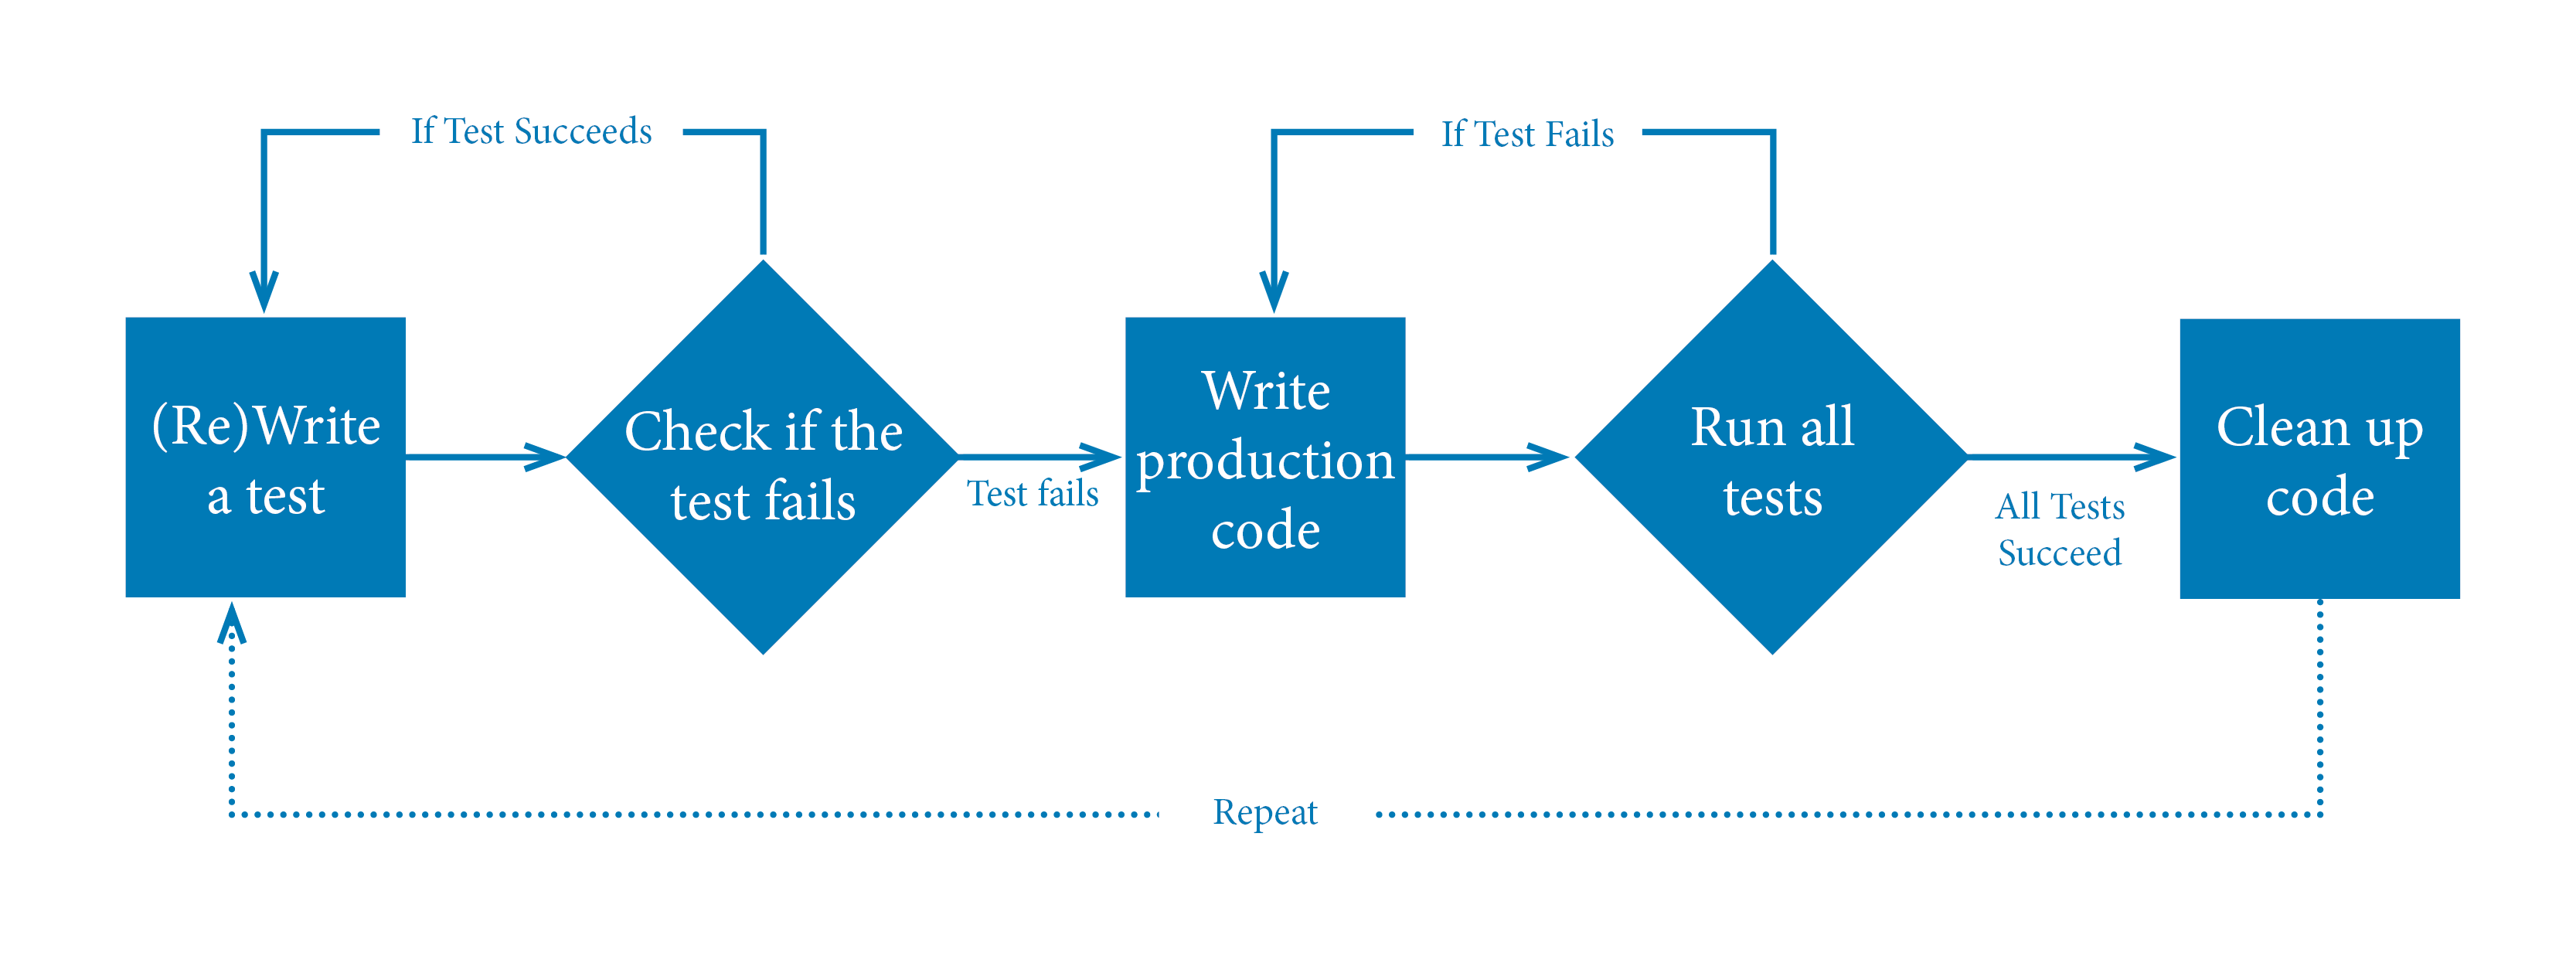
\includegraphics[width=\textwidth , keepaspectratio]{TestDrivenDevelopment.png}
\centering
\caption{Test Driven Development.} 
\source{\href{https://www.andplus.com/}{Andplus.com}}
\label{fig:tdd}
\end{figure}
In secondo luogo, ho configurato, tramite il \textit{framework} Jenkins, una \textit{pipeline} per la \textit{continuous integration} che eseguisse in maniera automatica i test precedentemente codificati.
Infine adottato il \textit{framework} \textbf{Swagger.io} per la documentazione delle chiamate \textit{API}.
%%%%%%%%%%%%%%%%%%%%%%%%%%%%%%%%%%%%%%%%%%%%%%%%%%%%%%%%%%%%%%%%%%%%%%%%%%%%%%%%%%%%%%%%%%%
\subsection{Vincoli tecnologici}
%stack tecnologico definito in avvio di progetto 

Per la realizzazione dei due progetti di stage, ho utilizzato due \textit{stack} tecnologici molto simili, ma per certi aspetti radicalmente differenti.\\
Il progetto \textbf{AWMS} si basa su tecnologie ampiamente utilizzate in azienda: 
\begin{itemize}
\item \textbf{PostgreSQL:} database relazionale, compatibile con il paradigma SQL, che consente all'utente di immagazinare dati anche in formato Json, rendendo di fatto il contenuto delle tabelle molto più dinamico;
\item \textbf{CakePHP:} \textit{framework} che consente lo sviluppo rapido di applicazioni web con architettura MVC. Grazie alla sua funzione di \textit{ORM}, permette di effettuare operazioni sulle tabelle trattando quest'ultime come oggetti derivanti dal paradigma \textit{OOP};
\item \textbf{Angular2+:} \textit{framework} per lo sviluppo di applicazioni web \textit{single-page}.
\end{itemize}
\textbf{DigitalSnapshots} invece si differenzia da AWMS in quanto sostituisce \textbf{MySQL} a \textit{PostgreSQL} e \textbf{AngularJS} ad \textit{Angular2+}.\\
Questa differenza di comparto tecnico è giustificata dal fatto che, mentre AWMS verrà seguito da \AD{} (nello specifico, da \textbf{I4.0Saas} dal 2020) per tutto il suo ciclo di vita, \textbf{DigitalSnapshots} avrà un destino differente: le fasi di progettazione e sviluppo sono a carico di \AD{}, mentre la fase di manutenzione del codice sarà eseguita dal reparto tecnico di Electrolux, committente del progetto.\\
Dai vincoli metodologici personali, deriva l'utilizzo dei \textit{framework} \textit{Jenkins}, per l'implementazione della \textit{continous integration}, e \textit{PHPUnit} e \textit{Jasmine} per l'esecuzione automatica dei test d'unità ed integrazione, rispettivamente per i linguaggi di programmazione PHP e Typescript.
\section{Aspettative personali}
%- come ho conosciuto AD\\
%- perchè AD?\\
%- aspettative sul lavorare in una startup, imparare il way of working\\
Durante l'ultimo anno del mio percorso accademico, ho avuto l'opportunità di partecipare a \textit{Stage-IT}, un evento organizzato da Assindustria Venetocentro in collaborazione con l'Università di Padova, con lo scopo di fornire un punto di contatto tra gli studenti e le aziende del settore informatico presenti nel territorio.
E\` proprio durante questo incontro che ho conosciuto \AD , e subito sono rimasto intrigato dalla sua dinamicità e propensione all'innovazione, nonché dai progetti ambiziosi e dai valori aziendali nei quali mi identifico.\\
\begin{figure}[h]

\includegraphics[width=\textwidth]{startup.jpg}
\centering
\caption{Le molte sfaccettature delle start-up.} 
\source{\href{http://orizzonti.tv/}{Orizzonti.tv}}
\label{fig:tdd}
\end{figure}
Le mie aspettative riguardo a questa attività di stage potevano essere riassunte in tre punti fondamentali:
\begin{itemize}
\item Innanzitutto, vedevo questo tirocinio come un banco di prova su cui testare le conoscenze acquisite durante il percorso universitario e la mia capacità di apprendimento di tecnologie a me perlopiù sconosciute;
\item In secondo luogo, ero smanioso di collaborare con aziende dal marchio rinomato, come Electrolux e Safilo.
\item Infine, ma non per questo meno importante, desideravo imparare il \textit{way of working} da persone con esperienza nel settore, perchè credo che conoscere gli strumenti e saperli utilizzare al meglio sia fondamentale per uno sviluppatore, specie se inesperto.
\end{itemize}
%%%%%%%%%%%%%%%%%%%%%%%%%%%%%%%%%%%%%%%%%%%%%%%%%%%%%%%%%%%%%%%%%%%%%%%%%%%%%%%%%%%%%%%%%%%             % Processi
% !TEX encoding = UTF-8
% !TEX TS-program = pdflatex
% !TEX root = ../tesi.tex

%**************************************************************
\chapter{Descrizione dello stage}
\label{cap:descrizione-stage}
%**************************************************************

\intro{Breve introduzione al capitolo}\\

%**************************************************************
\section{Introduzione al progetto}

%**************************************************************
\section{Analisi preventiva dei rischi}

Durante la fase di analisi iniziale sono stati individuati alcuni possibili rischi a cui si potrà andare incontro.
Si è quindi proceduto a elaborare delle possibili soluzioni per far fronte a tali rischi.\\

\begin{risk}{Performance del simulatore hardware}
    \riskdescription{le performance del simulatore hardware e la comunicazione con questo potrebbero risultare lenti o non abbastanza buoni da causare il fallimento dei test}
    \risksolution{coinvolgimento del responsabile a capo del progetto relativo il simulatore hardware}
    \label{risk:hardware-simulator} 
\end{risk}

%**************************************************************
\section{Requisiti e obiettivi}


%**************************************************************
\section{Pianificazione}             % Kick-Off
% !TEX encoding = UTF-8
% !TEX TS-program = pdflatex
% !TEX root = ../tesi.tex
%**************************************************************
\cleardoublepage
\chapter{Valutazione retrospettiva}
\label{cap:valutazione-retrospettiva}
%**************************************************************
\section{Bilancio degli obiettivi raggiunti}
- tabella che indica gli obiettivi soddisfatti e non soddisfatti \\
- spiegazione degli obiettivi non soddisfatti\\
- bilancio degli obiettivi personali
%**************************************************************
\section{Conoscenze e competenze acquisite}
- competenze tecniche (linguaggi di programmazione, utilizzo dei tool di lavoro)\\
- competenze progettuali (punti di forza e limiti di alcune soluzioni rispetto ad altre)\\
- esperienza professionale\\

\section{Valutazione personale}
- difficile approccio con Angular in quanto javascript/typescript è stato poco trattato durante il corso accademico. Fortunatamente, l'architettura MVC mi era già nota, e questo ha facilitato un po' la comprensione del suo funzionamento\\
- il corso accademico dovrebbe fornire agli studenti una base sugli strumenti di supporto allo sviluppo più comuni (versionamento, framework di testing, CI/CD)             % Concept Preview
% !TEX encoding = UTF-8
% !TEX TS-program = pdflatex
% !TEX root = ../tesi.tex

%**************************************************************
\chapter{Progettazione e codifica}
\label{cap:progettazione-codifica}
%**************************************************************

\intro{Breve introduzione al capitolo}\\

%**************************************************************
\section{Tecnologie e strumenti}
\label{sec:tecnologie-strumenti}

Di seguito viene data una panoramica delle tecnologie e strumenti utilizzati.

\subsection*{Tecnologia 1}
Descrizione Tecnologia 1.

\subsection*{Tecnologia 2}
Descrizione Tecnologia 2

%**************************************************************
\section{Ciclo di vita del software}
\label{sec:ciclo-vita-software}

%**************************************************************
\section{Progettazione}
\label{sec:progettazione}

\subsubsection{Namespace 1} %**************************
Descrizione namespace 1.

\begin{namespacedesc}
    \classdesc{Classe 1}{Descrizione classe 1}
    \classdesc{Classe 2}{Descrizione classe 2}
\end{namespacedesc}


%**************************************************************
\section{Design Pattern utilizzati}

%**************************************************************
\section{Codifica}
             % Product Prototype
% !TEX encoding = UTF-8
% !TEX TS-program = pdflatex
% !TEX root = ../tesi.tex

%**************************************************************
\chapter{Verifica e validazione}
\label{cap:verifica-validazione}
%**************************************************************             % Product Design Freeze e SOP
% !TEX encoding = UTF-8
% !TEX TS-program = pdflatex
% !TEX root = ../tesi.tex

%**************************************************************
\chapter{Conclusioni}
\label{cap:conclusioni}
%**************************************************************

%**************************************************************
\section{Consuntivo finale}

%**************************************************************
\section{Raggiungimento degli obiettivi}

%**************************************************************
\section{Conoscenze acquisite}

%**************************************************************
\section{Valutazione personale}
             % Conclusioni
\appendix                               
% !TEX encoding = UTF-8
% !TEX TS-program = pdflatex
% !TEX root = ../tesi.tex

%**************************************************************
\chapter{Appendice A}
%**************************************************************

\epigraph{Citazione}{Autore della citazione}



             % Appendice A

%**************************************************************
% Materiale finale
%**************************************************************
\backmatter
\printglossaries
% !TEX encoding = UTF-8
% !TEX TS-program = pdflatex
% !TEX root = ../tesi.tex

%**************************************************************
% Bibliografia
%**************************************************************

\cleardoublepage
\chapter{Bibliografia}

\nocite{*}
% Stampa i riferimenti bibliografici
\printbibliography[heading=subbibliography,title={Riferimenti bibliografici},type=book]

% Stampa i siti web consultati
\printbibliography[heading=subbibliography,title={Siti web consultati},type=online]


\end{document}
